%%=============================================================================
%% Methodologie
%%=============================================================================

\chapter{\IfLanguageName{dutch}{Methodologie}{Methodology}}%
\label{ch:methodologie}

% TODO: In dit hoofstuk geef je een korte toelichting over hoe je te werk bent
% gegaan. Verdeel je onderzoek in grote fasen, en licht in elke fase toe wat
% de doelstelling was, welke deliverables daar uit gekomen zijn, en welke
% onderzoeksmethoden je daarbij toegepast hebt. Verantwoord waarom je
% op deze manier te werk gegaan bent.

% Voorbeelden van zulke fasen zijn: literatuurstudie, opstellen van een
% requirements-analyse, opstellen long-list (bij vergelijkende studie),
% selectie van geschikte tools (bij vergelijkende studie, "short-list"),
% opzetten testopstelling/PoC, uitvoeren testen en verzamelen
% van resultaten, analyse van resultaten, ...

% !!!!! LET OP !!!!!

% Het is uitdrukkelijk NIET de bedoeling dat je het grootste deel van de corpus
% van je graduaatsproef in dit hoofstuk verwerkt! Dit hoofdstuk is eerder een
% kort overzicht van je plan van aanpak.

% Maak voor elke fase (behalve het literatuuronderzoek) een NIEUW HOOFDSTUK aan
% en geef het een gepaste titel.


The research will be conducted by creating a proof-of-concept application and studying online documentation of certain frameworks. Writing thesis by developing software solution is not only a task that requires knowledge of programming languages, but also technical skills, so it can only be done by people with IT background. The project will be made on a PC laptop running Linux system and Windows on virtual machine. The code will be written in Visual Studio Code \autocite{Vscode}, along with extensions dedicated to TypeScript and Vue. It will be also necessary to use Android emulator for testing mobile version of the application. Development changes will be tracked using Git version control system and documented in an Azure DevOps project bind with a Github \autocite{Github} repository. 
Git commits contain an annotation referring to the specific Epics, Features, User-Stories, Tasks or Bugs numbers according to the Azure Boards format \autocite{AzureBoards}.

The work is devided into main phases:

\begin{itemize}
    \item Research and analys of existing cross-platform solutions
    \item Developing a working proof-of-concept application, including layout, domain and architecture design, implementing functionalities
    \item Implementing synchronization between client applications
    \item Results analysys, finding benefits and difficulties
\end{itemize}

\begin{figure}[H]
    \centering
    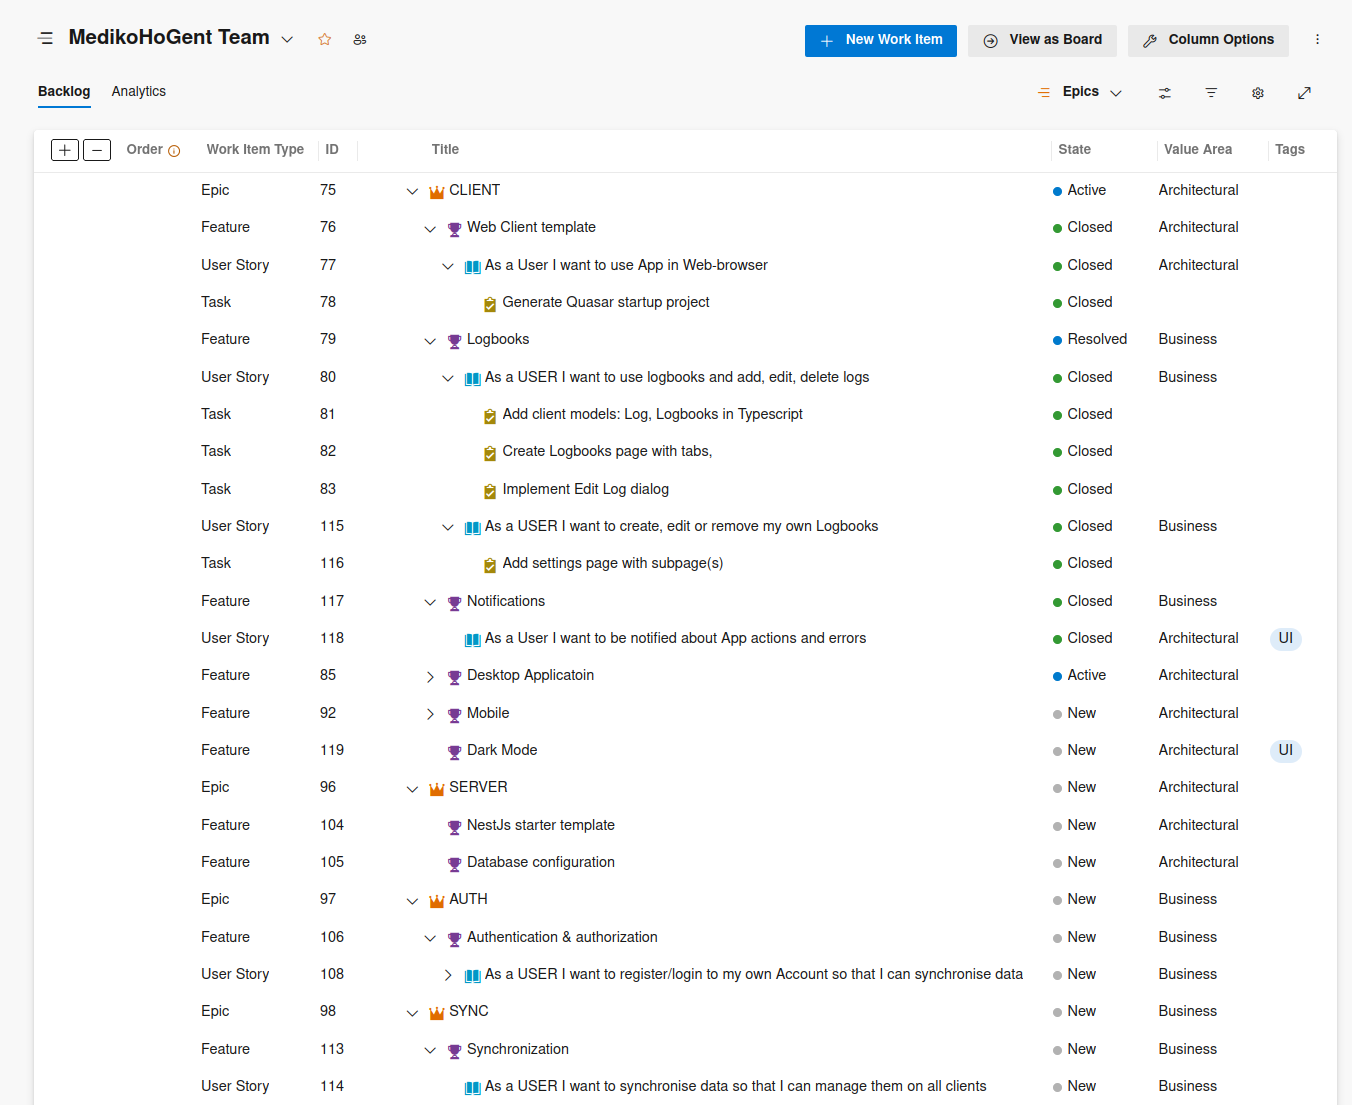
\includegraphics[width=0.8\textwidth]{azure-backlog}
    \caption[Azure DevOps backlog page]{\label{fig:azuredevops} Azure DevOps backlog page }
\end{figure}